\documentclass[aspectratio=169,12pt]{beamer}
\usetheme{Madrid}
\usecolortheme{dolphin}
\usefonttheme{professionalfonts}
\setbeamertemplate{navigation symbols}{}
\setbeamertemplate{footline}{}

\usepackage[T1]{fontenc}
\usepackage[utf8]{inputenc}
\usepackage{graphicx}
\usepackage{amsmath,amssymb}
\usepackage{hyperref}
\usepackage{siunitx}
\usepackage{physics}

\graphicspath{{../../figures/}}

\title[Module A2]{Module A2: Le qubit (sans nombres complexes)}
\author{JAMOTTE Maxime, SCHOONEN Cédric}
\institute{Digital Learning Hub}
\date{}

\begin{document}

\begin{frame}
  \titlepage
\end{frame}

\begin{frame}{Objectifs du module A2}
  \begin{enumerate}
    \item Représentation vectorielle\\~\\
    \item Représentation bra-ket\\~\\
    \item Superposition et lien entre probabilité et coefficients\\~\\
    \item Les matrices et leur action sur les vecteurs\\~\\
    \item Opérations sur un qubit : $X$, $Z$, $H$
  \end{enumerate}
\end{frame}

% ============================================================
\section{Représentation vectorielle}
% ============================================================

\begin{frame}{Vecteurs}
  {%
    \setbeamercolor{itemize/enumerate body}{fg=gray!60}
    \setbeamercolor{itemize item}{fg=gray!60}
    \setbeamercolor{alerted text}{fg=black}
    \begin{columns}[T]
      \begin{column}{0.55\textwidth}
        \begin{itemize}[<+-| alert@+>]
          \setlength{\itemsep}{0.6em}
          \item Définition d'un vecteur
          \item Addition de vecteurs
          \item Multiplication d'un vecteur par une constante
        \end{itemize}
        \bigskip
        \only<1>{\[
          \vec r = \begin{pmatrix} a \\ b \end{pmatrix}
        \]}
        \only<2>{\[
          \vec r + \vec p = 
          \begin{pmatrix} a \\ b \end{pmatrix} +
          \begin{pmatrix} c \\ d \end{pmatrix} =
          \begin{pmatrix} a+c \\ b+d \end{pmatrix}
        \]}
        \only<3>{\[
          \lambda \begin{pmatrix} a \\ b \end{pmatrix} =
          \begin{pmatrix} \lambda a \\ \lambda b \end{pmatrix}
        \]}
      \end{column}
      \begin{column}{0.4\textwidth}
        \centering
        \only<1>{
\includegraphics[width=\linewidth]{vecteur.png}}
        \only<2>{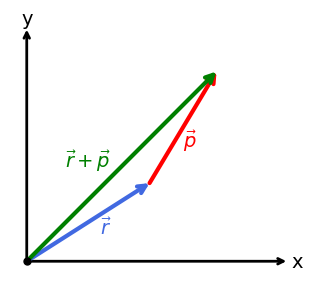
\includegraphics[width=\linewidth]{add_vecteurs.png}}
        \only<3->{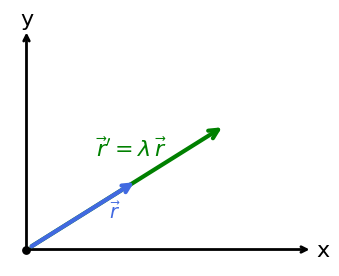
\includegraphics[width=\linewidth]{multiplication_nombre.png}}
      \end{column}
    \end{columns}
  }
\end{frame}

% ============================================================
\section{Représentation bra-ket}
% ============================================================

\begin{frame}{Qubit}
  \begin{itemize}[<+->]
    \setlength{\itemsep}{0.6em}
    \item L'électron passe à travers les fentes du haut ($H$) et du bas ($B$) en même temps.
      \only<1->{%
        \vspace{0.5em}
        \begin{center}
          \begin{minipage}{0.42\textwidth}
            \centering
            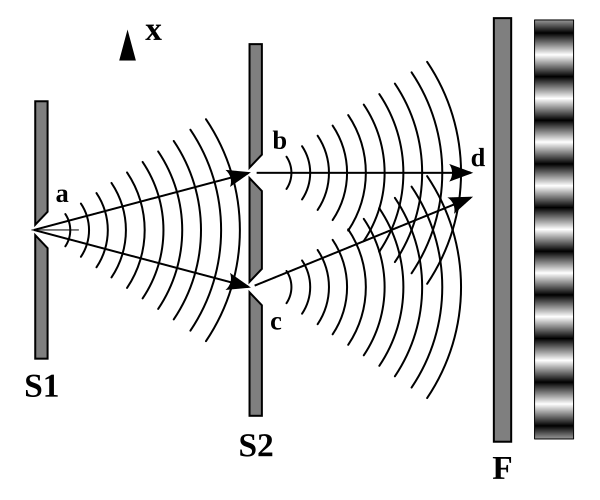
\includegraphics[width=0.6\linewidth]{fente_Young.png}
          \end{minipage}\hfill
          \begin{minipage}{0.42\textwidth}
            \centering
            \only<2->{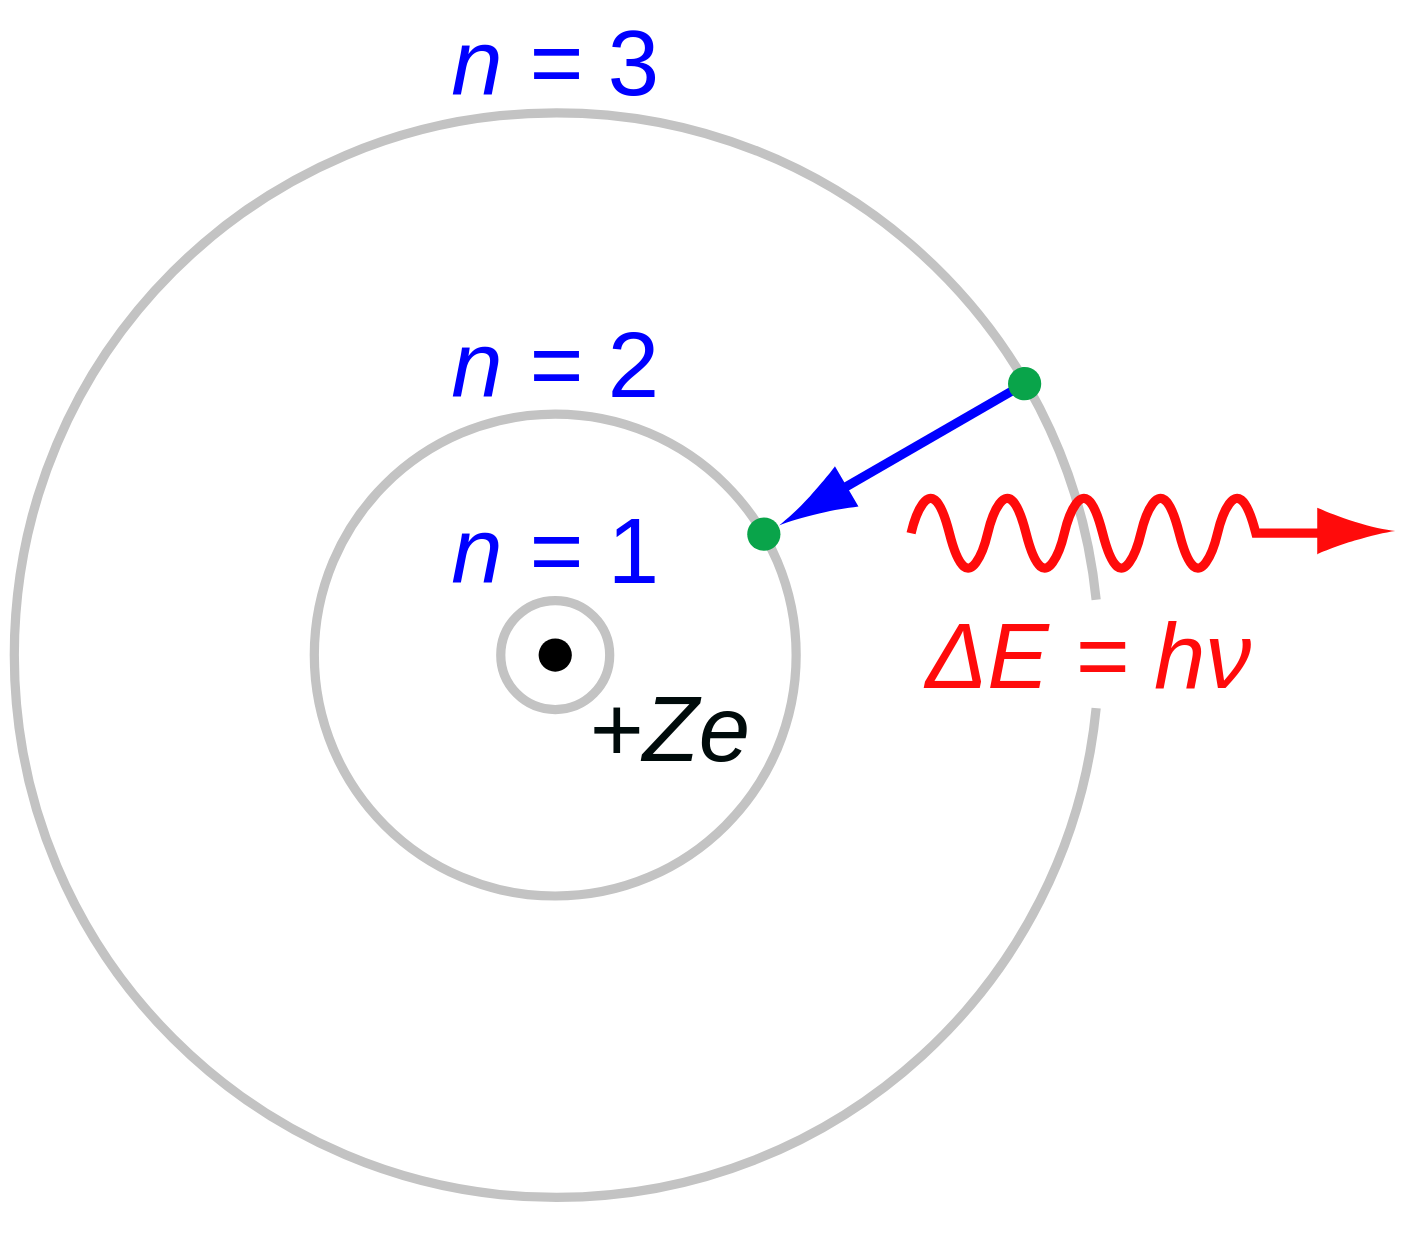
\includegraphics[width=0.6\linewidth]{bohr_model.png}}
          \end{minipage}
        \end{center}
      }
    \item Certains systèmes physiques ont des niveaux discrets d'énergie (au lieu de la position).
    \item \textbf{Qubit} (= bit quantique) = système quantique à 2 niveaux, notés $\ket 0$ et $\ket 1$.
  \end{itemize}
\end{frame}

% ============================================================
\section{Superposition et probabilités}
% ============================================================

\begin{frame}{Superposition d'états et vecteurs}
  \begin{columns}[T]
    \begin{column}{0.65\textwidth}
      \begin{itemize}[<+->]
        \item Un qubit peut être dans $\ket 0$, $\ket 1$ ou toute \textbf{superposition} des deux: $\alpha \ket 0 + \beta \ket 1$.
        \item Superposition = combinaison linéaire d'états.
        \item \textbf{Postulat} : les états quantiques forment un espace vectoriel (espace de Hilbert). Une combinaison linéaire d'états est aussi un état.
        \item L'état superposé $\ket {\psi} = \alpha \ket 0 + \beta \ket 1$, s'écrit $\begin{pmatrix} \alpha \\ \beta \end{pmatrix}$,\\~\\
        \item Chaque \textbf{qubit} est identifiable à la \textbf{direction} de son vecteur.
        \item Si deux vecteurs ont la \textbf{même direction} ($\theta = 0$), leurs qubits occupent le \textbf{même état}.
      \end{itemize}
    \end{column}
    \begin{column}{0.35\textwidth}
      \vspace{2em}
      \centering
      $\ket 0 = \begin{pmatrix}1 \\ 0\end{pmatrix}$ et $\ket 1 = \begin{pmatrix}0 \\ 1\end{pmatrix}$\\~\\~\\
      \only<4->{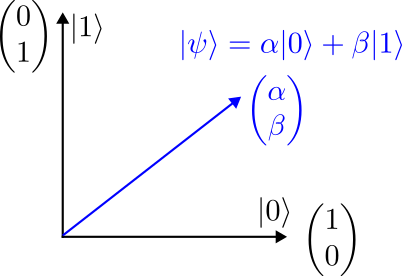
\includegraphics[width=0.8\textwidth]{ket_base.png}}
    \end{column}
  \end{columns}
\end{frame}

% ============================================================
\section{Les matrices}
% ============================================================

\begin{frame}{Les matrices et leur action sur un vecteur}
  {%
    \setbeamercolor{itemize/enumerate body}{fg=gray!60}
    \setbeamercolor{itemize item}{fg=gray!60}
    \setbeamercolor{alerted text}{fg=black}
    \begin{columns}[T]
      \begin{column}{0.55\textwidth}
        \begin{itemize}[<+-| alert@+>]
          \setlength{\itemsep}{0.6em}
          \item Multiplication matrice-vecteur
          \item Addition de matrices
          \item Multiplication d'une matrice par un scalaire
        \end{itemize}
        \bigskip
        \only<1>{\[M \vec{r} = 
          \begin{pmatrix} a & b \\ c & d \end{pmatrix}
          \begin{pmatrix} u \\ v \end{pmatrix} =
          \begin{pmatrix} au + bv \\ cu + dv \end{pmatrix}
        \]}
      \end{column}
      \begin{column}{0.4\textwidth}
        \centering
        \only<1>{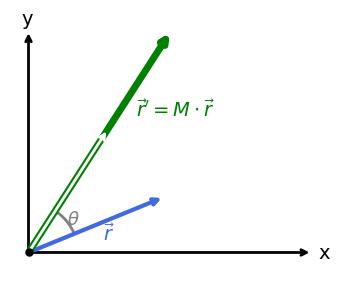
\includegraphics[width=\linewidth]{multiplication_Mv.png}}
        \only<2>{\fbox{\Large $M_1^{}+M_2^{}$}}
        \only<3>{\fbox{\Large $\lambda M$}}
      \end{column}
    \end{columns}
        \only<2>{\[M_1^{}+M_2^{} = 
          \begin{pmatrix} a & b\\ c & d \end{pmatrix} +
          \begin{pmatrix} e & f\\ g & h \end{pmatrix} =
          \begin{pmatrix} a+e & b+f\\ c+g & d+h \end{pmatrix}
        \]}
        \only<3>{\[ \lambda M = 
          \lambda \begin{pmatrix} a & b\\ c & d \end{pmatrix} =
          \begin{pmatrix} \lambda a & \lambda b\\ \lambda c & \lambda d \end{pmatrix}
        \]}
  }
\end{frame}

\begin{frame}{Multiplication de deux matrices}
  \[ M_1^{} \times M_2^{} = \begin{pmatrix}
      a & b \\
      c & d
    \end{pmatrix}
    \begin{pmatrix}
      u_1^{} & u_2^{} \\
      v_1^{} & v_2^{}
    \end{pmatrix}
    =
    \begin{pmatrix}
      au_1^{} + bv_1^{} & au_2^{} + bv_2^{} \\
      cu_1^{} + dv_1^{} & cu_2^{} + dv_2^{}
    \end{pmatrix}
  \]
  \\~\\
    \textbf{Non commutatif} en général : $M_1^{} \times M_2^{} \neq M_2^{} \times M_1^{}$.
  
  \bigskip
  \[
    \begin{pmatrix}
      0 & 1 \\
      1 & 0
    \end{pmatrix}
    \begin{pmatrix}
      1 & 0 \\
      0 & -1
    \end{pmatrix}
    =
    \begin{pmatrix}
      0 & -1 \\
      1 & 0
    \end{pmatrix}
      \]
  \bigskip
  \[
    \begin{pmatrix}
      1 & 0 \\
      0 & -1
    \end{pmatrix}
    \begin{pmatrix}
      0 & 1 \\
      1 & 0
    \end{pmatrix}
    =
    \begin{pmatrix}
      0 & 1 \\
      -1 & 0
    \end{pmatrix}
  \]
\end{frame}

% ============================================================
\section{Opérations sur un qubit}
% ============================================================

\begin{frame}{Les matrices décrivent les opérations sur les qubits}
  \begin{itemize}[<+->]
    \setlength{\itemsep}{0.6em}
    \item Les matrices ne sont pas qu'un objet mathématique abstrait :
      en mécanique quantique, chaque \textbf{opération physique} sur un qubit
      correspond à une matrice.
    \item Un état $\ket{\psi}$ transformé par une opération $U$ donne
      $\ket{\psi'} = U\ket{\psi}$.
    \item Voyons trois opérations fondamentales à~1~qubit~: $X$, $Z$ et $H$.
  \end{itemize}
\end{frame}

\begin{frame}{Porte $X$ (bit-flip)}
  \begin{columns}[T]
    \begin{column}{0.55\textwidth}
      \[ X = \begin{pmatrix} 0 & 1 \\ 1 & 0 \end{pmatrix} \]
      \begin{itemize}[<+->]
        \setlength{\itemsep}{0.6em}
        \item $X\ket{0} = \ket{1}$, \quad $X\ket{1} = \ket{0}$.
        \item Analogue quantique du \texttt{NOT} classique.
        \item Échange les coefficients $\alpha$ et $\beta$.
      \end{itemize}
    \end{column}
    \begin{column}{0.4\textwidth}
      \centering
      \includegraphics[width=0.8\linewidth]{X.png}
    \end{column}
  \end{columns}
\end{frame}

\begin{frame}{Porte $Z$ (phase-flip)}
  \begin{columns}[T]
    \begin{column}{0.55\textwidth}
      \[ Z = \begin{pmatrix} 1 & 0 \\ 0 & -1 \end{pmatrix} \]
      \begin{itemize}[<+->]
        \setlength{\itemsep}{0.6em}
        \item $Z\ket{0} = \ket{0}$, \quad $Z\ket{1} = -\ket{1}$.
        \item Change le signe relatif entre $\ket{0}$ et $\ket{1}$.
        \item Aucun équivalent classique (pas de changement de probabilités).
      \end{itemize}
    \end{column}
    \begin{column}{0.4\textwidth}
      \centering
      \includegraphics[width=0.8\linewidth]{Z.png}
    \end{column}
  \end{columns}
\end{frame}

\begin{frame}{Porte de Hadamard $H$}
  \begin{columns}[T]
    \begin{column}{0.55\textwidth}
      \[ H = \frac{1}{\sqrt{2}} \begin{pmatrix} 1 & 1 \\ 1 & -1 \end{pmatrix} \]
      \begin{itemize}[<+->]
        \setlength{\itemsep}{0.6em}
        \item $H\ket{0} = \frac{1}{\sqrt{2}}(\ket{0}+\ket{1}) \equiv \ket{+}$.
        \item $H\ket{1} = \frac{1}{\sqrt{2}}(\ket{0}-\ket{1}) \equiv \ket{-}$.
        \item Crée une superposition 50/50 à partir d'un état de base.
      \end{itemize}
    \end{column}
    \begin{column}{0.4\textwidth}
      \centering
      \includegraphics[width=0.8\linewidth]{H.png}
    \end{column}
  \end{columns}
\end{frame}

\begin{frame}{Fin du module A2}
  \begin{enumerate}
    \item Représentation vectorielle\\~\\
    \item Représentation bra-ket\\~\\
    \item Superposition et lien entre probabilité et coefficients\\~\\
    \item Les matrices et leur action sur les vecteurs\\~\\
    \item Opérations sur un qubit : $X$, $Z$, $H$
  \end{enumerate}
\end{frame}

\end{document}
